\section{Piani di accesso}
\subsection{Piani di accesso logico}
Stampare codice, nome e valutazione degli esami sostenuti dallo
studente con matricola '278233'.
\begin{center}
	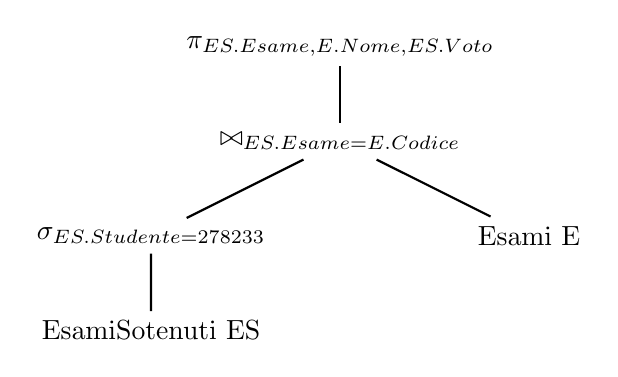
\begin{tikzpicture}[scale=0.8]
		\node (M) at (-3, 0) {EsamiSotenuti ES};
		\node (R) at (3, 1.5) {Esami E};
		\node (mrb) at (-3, 1.5) {$\sigma_\text{ES.Studente = 278233}$};
		\node (j) at (0, 3) {$\bowtie_\text{ES.Esame = E.Codice}$};
		\node (pc) at (0, 4.5) {$\pi_\text{ES.Esame, E.Nome, ES.Voto}$};

		\path (M) edge[thick] (mrb)
		(mrb) edge[thick] (j)
		(R) edge[thick] (j)
		(j) edge[thick] (pc);
	\end{tikzpicture}
\end{center}
Seleziona gli accounti attivi degli studenti che hanno gli
stessi nomi e cognomi e li stampa in ordine alfabetico.
\begin{center}
	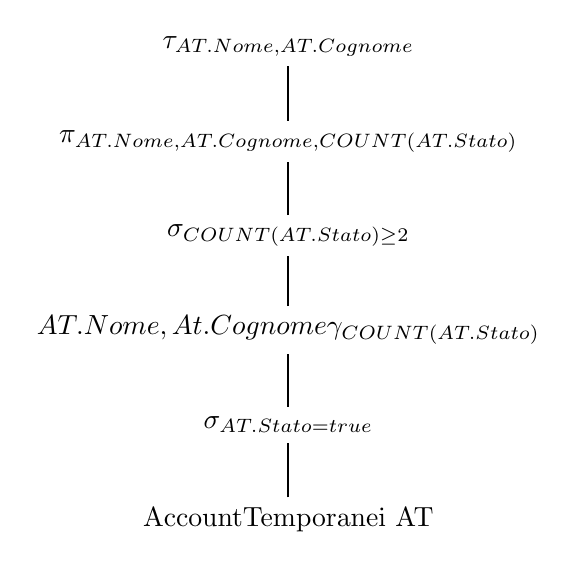
\begin{tikzpicture}[scale=0.8]
		\node (M) at (0, 0) {AccountTemporanei AT};
		\node (plastica) at (0, 1.5) {$\sigma_\text{AT.Stato = true}$};
		\node (group) at (0, 3) {$\prescript{}{\text{AT.Nome, At.Cognome}}{\gamma}_\text{COUNT(AT.Stato)}$};
		\node (having) at (0, 4.5) {$\sigma_{\text{COUNT(AT.Stato)} \geq 2}$};
		\node (projection) at (0, 6) {$\pi_\text{AT.Nome, AT.Cognome, COUNT(AT.Stato)}$};
		\node (order) at (0, 7.5) {$\tau_\text{AT.Nome, AT.Cognome}$};

		\path (M) edge[thick] (plastica);
		\path (plastica) edge[thick] (group);
		\path (group) edge[thick] (having);
		\path (having) edge[thick] (projection);
		\path (projection) edge[thick] (order);
	\end{tikzpicture}
\end{center}
Stampa matricola, nome completo e media degli studenti la cui
media è superiore a 27.
\begin{center}
	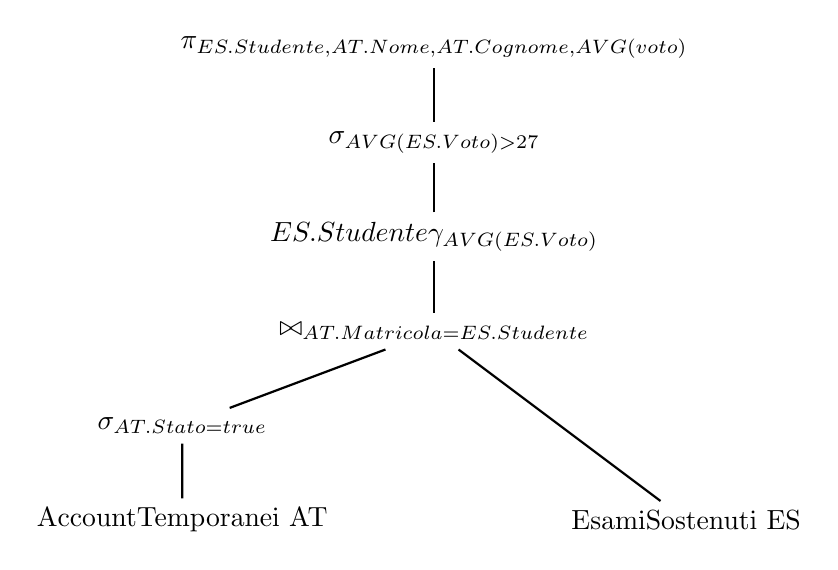
\begin{tikzpicture}[scale=0.8]
		\node (P) at (-4, 0) {AccountTemporanei AT};
		\node (PM) at (4, 0) {EsamiSostenuti ES};
		\node (join) at (-4, 1.5) {$\sigma_\text{AT.Stato = true}$};
		\node (nero) at (0, 3) {$\bowtie_\text{AT.Matricola = ES.Studente}$};
		\node (group) at (0, 4.5) {$\prescript{}{\text{ES.Studente}}{\gamma}_\text{AVG(ES.Voto)}$};
		\node (having) at (0, 6) {$\sigma_{\text{AVG(ES.Voto)} > 27}$};
		\node (projection) at (0, 7.5) {$\pi_\text{ES.Studente, AT.Nome, AT.Cognome, AVG(voto)}$};

		\path (P) edge[thick] (join)
		(PM) edge[thick] (nero)
		(join) edge[thick] (nero)
		(nero) edge[thick] (group)
		(group) edge[thick] (having)
		(having) edge[thick] (projection);
	\end{tikzpicture}
\end{center}

\subsection{Piani di accesso fisico senza indice}
Stampare codice, nome e valutazione degli esami sostenuti dallo
studente con matricola '278233'.
\begin{center}
	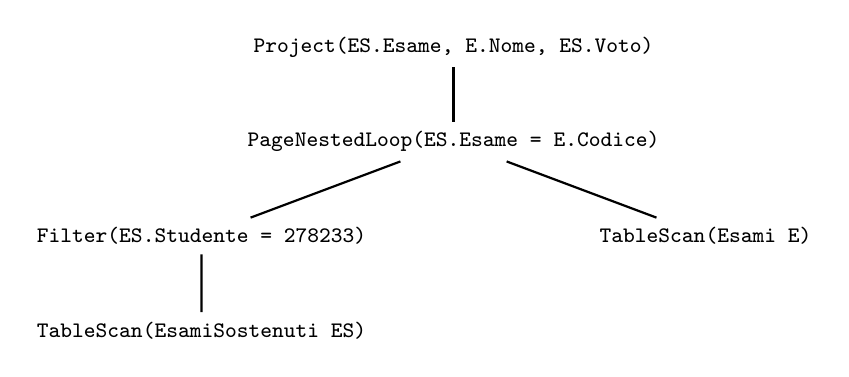
\begin{tikzpicture}[scale=0.8, font=\footnotesize]
		\node (M) at (-4, 0) {\verb|TableScan(EsamiSostenuti ES)|};
		\node (R) at (4, 1.5) {\verb|TableScan(Esami E)|};
		\node (mrb) at (-4, 1.5) {\verb|Filter(ES.Studente = 278233)|};
		\node (j) at (0, 3) {\verb|PageNestedLoop(ES.Esame = E.Codice)|};
		\node (pc) at (0, 4.5) {\verb|Project(ES.Esame, E.Nome, ES.Voto)|};

		\path (M) edge[thick] (mrb)
		(mrb) edge[thick] (j)
		(R) edge[thick] (j)
		(j) edge[thick] (pc);
	\end{tikzpicture}
\end{center}
Seleziona gli account attivi degli studenti che hanno gli
stessi nomi e cognomi e li stampa in ordine alfabetico.
\begin{center}
	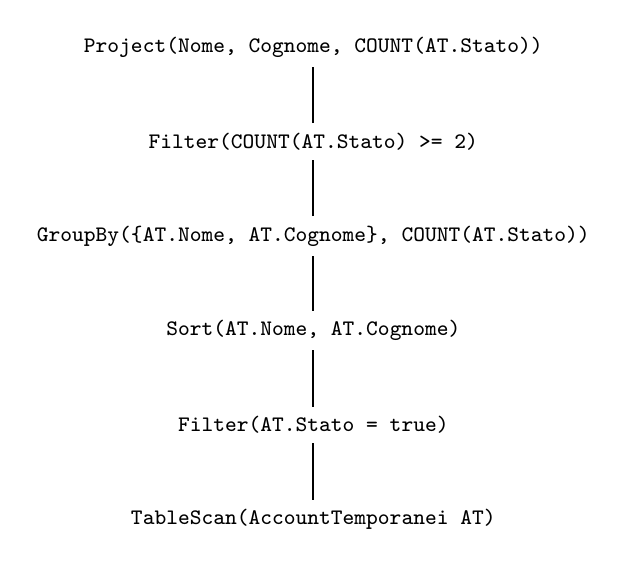
\begin{tikzpicture}[scale=0.8, font=\footnotesize]
		\node (M) at (0, 0) {\verb|TableScan(AccountTemporanei AT)|};
		\node (stato) at (0, 1.5) {\verb|Filter(AT.Stato = true)|};
		\node (sort1) at (0, 3) {\verb|Sort(AT.Nome, AT.Cognome)|};
		\node (group) at (0, 4.5) {\verb|GroupBy({AT.Nome, AT.Cognome}, COUNT(AT.Stato))|};
		\node (having) at (0, 6) {\verb|Filter(COUNT(AT.Stato) >= 2)|};
		\node (projection) at (0, 7.5) {\verb|Project(Nome, Cognome, COUNT(AT.Stato))|};


		\path (M) edge[thick] (stato);
		\path (stato) edge[thick] (sort1);
		\path (sort1) edge[thick] (group);
		\path (group) edge[thick] (having);
		\path (having) edge[thick] (projection);
	\end{tikzpicture}
\end{center}
Stampa matricola, nome completo e media degli studenti la cui
media è superiore a 27.
\begin{center}
	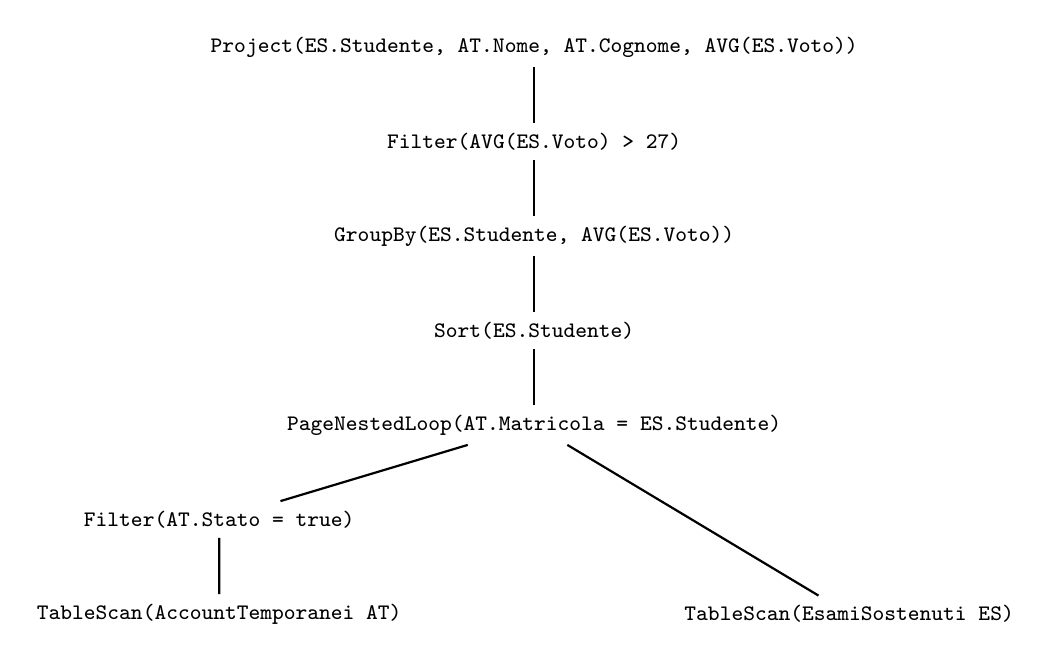
\begin{tikzpicture}[scale=0.8, font=\footnotesize]
		\node (P) at (-5, 0) {\verb|TableScan(AccountTemporanei AT)|};
		\node (PM) at (5, 0) {\verb|TableScan(EsamiSostenuti ES)|};
		\node (join) at (0, 3) {\verb|PageNestedLoop(AT.Matricola = ES.Studente)|};
		\node (nero) at (-5, 1.5) {\verb|Filter(AT.Stato = true)|};
		\node (sort) at (0, 4.5) {\verb|Sort(ES.Studente)|};
		\node (group) at (0, 6) {\verb|GroupBy(ES.Studente, AVG(ES.Voto))|};
		\node (having) at (0, 7.5) {\verb|Filter(AVG(ES.Voto) > 27)|};
		\node (proj) at (0, 9) {\verb|Project(ES.Studente, AT.Nome, AT.Cognome, AVG(ES.Voto))|};

		\path (P) edge[thick] (nero)
		(PM) edge[thick] (join)
		(nero) edge[thick] (join)
		(join) edge[thick] (sort)
		(sort) edge[thick] (group)
		(group) edge[thick] (having)
		(having) edge[thick] (proj);
	\end{tikzpicture}
\end{center}
\subsection{Piani di accesso fisico con indice}
Stampare codice, nome e valutazione degli esami sostenuti dallo
studente con matricola '278233'.

\begin{center}
	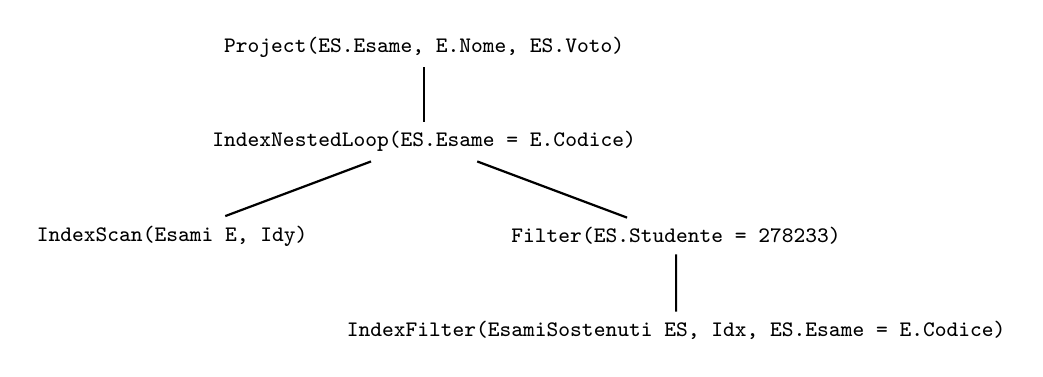
\begin{tikzpicture}[scale=0.8, font=\footnotesize]
		\node (TS) at (-4, 1.5) {\verb|IndexScan(Esami E, Idy)|};
		\node (IF) at (4, 0) {\verb|IndexFilter(EsamiSostenuti ES, Idx, ES.Esame = E.Codice)|};
		\node (F) at (4, 1.5) {\verb|Filter(ES.Studente = 278233)|};
		\node (INL) at (0, 3) {\verb|IndexNestedLoop(ES.Esame = E.Codice)|};
		\node (P) at (0, 4.5) {\verb|Project(ES.Esame, E.Nome, ES.Voto)|};

		\path (IF) edge[thick] (F)
		(TS) edge[thick] (INL)
		(F) edge[thick] (INL)
		(INL) edge[thick] (P);

	\end{tikzpicture}
\end{center}
Seleziona gli account attivi degli studenti che hanno gli
stessi nomi e cognomi e li stampa in ordine alfabetico.
\begin{center}
	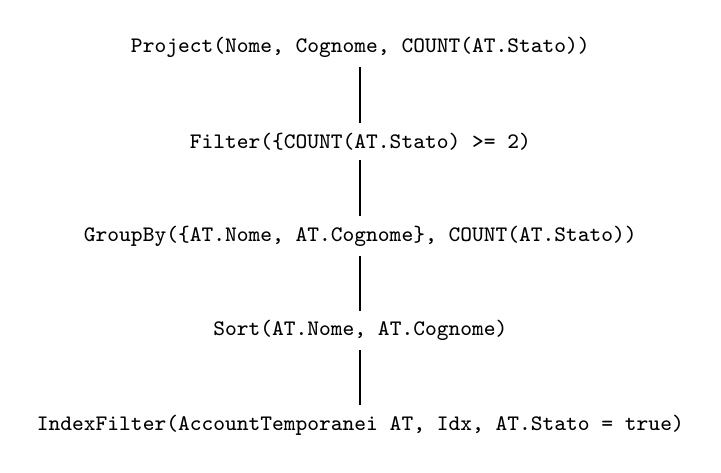
\begin{tikzpicture}[scale=0.8, font=\footnotesize]
		\node (M) at (0,0) {\verb|IndexFilter(AccountTemporanei AT, Idx, AT.Stato = true)|};
		\node (sort) at (0, 1.5) {\verb|Sort(AT.Nome, AT.Cognome)|};
		\node (groupby) at (0, 3) {\verb|GroupBy({AT.Nome, AT.Cognome}, COUNT(AT.Stato))|};
		\node (filter) at (0, 4.5) {\verb|Filter({COUNT(AT.Stato) >= 2)|};
		\node (project) at (0, 6) {\verb|Project(Nome, Cognome, COUNT(AT.Stato))|};


		\path (M) edge[thick] (sort);
		\path (sort) edge[thick] (groupby);
		\path (groupby) edge[thick] (filter);
		\path (filter) edge[thick] (project);
	\end{tikzpicture}
\end{center}
Stampa matricola, nome completo e media degli studenti la cui
media è superiore a 27.
\begin{center}
	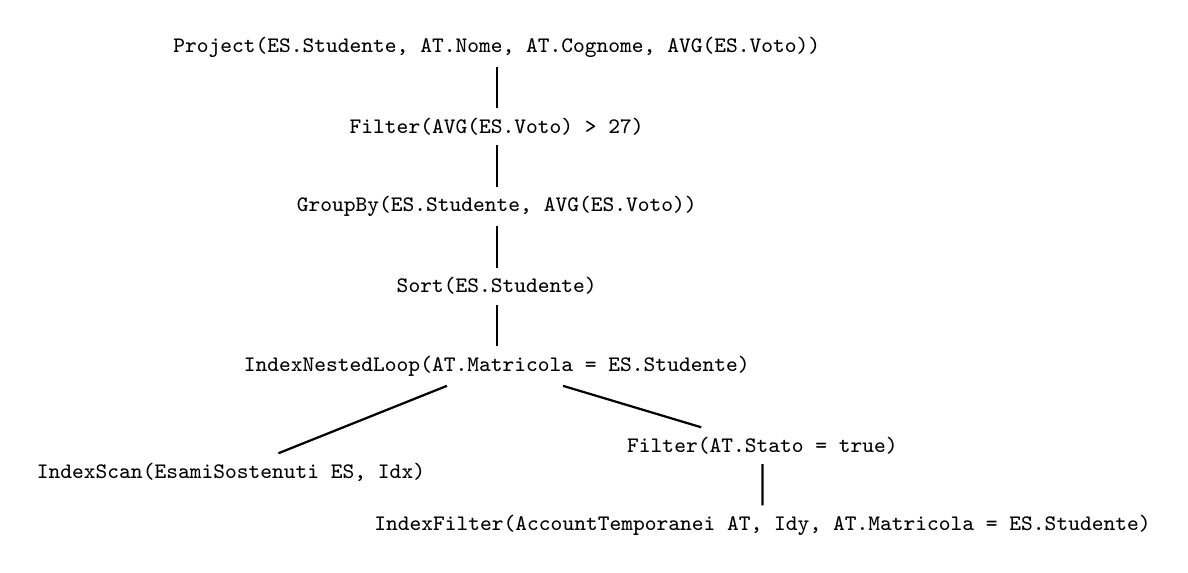
\begin{tikzpicture}[scale=0.675, font=\footnotesize]
		\node (P) at (5, 0) {\verb|IndexFilter(AccountTemporanei AT, Idy, AT.Matricola = ES.Studente)|};
		\node (PM) at (-5, 1) {\verb|IndexScan(EsamiSostenuti ES, Idx)|};
		\node (join) at (0, 3) {\verb|IndexNestedLoop(AT.Matricola = ES.Studente)|};
		\node (nero) at (5, 1.5) {\verb|Filter(AT.Stato = true)|};
		\node (sort) at (0, 4.5) {\verb|Sort(ES.Studente)|};
		\node (group) at (0, 6) {\verb|GroupBy(ES.Studente, AVG(ES.Voto))|};
		\node (having) at (0, 7.5) {\verb|Filter(AVG(ES.Voto) > 27)|};
		\node (proj) at (0, 9) {\verb|Project(ES.Studente, AT.Nome, AT.Cognome, AVG(ES.Voto))|};

		\path (P) edge[thick] (nero)
		(PM) edge[thick] (join)
		(nero) edge[thick] (join)
		(join) edge[thick] (sort)
		(sort) edge[thick] (group)
		(group) edge[thick] (having)
		(having) edge[thick] (proj);
	\end{tikzpicture}
\end{center}

% non so se si può evitare il sort prima della group by perchè non ho capito come funziona indexnestedloop. Domani lo guardo... come ultima cosa.
